\documentclass{article}
\usepackage{amssymb}
\usepackage{amsmath}
\usepackage{amsthm}
\usepackage{tikz}
\usepackage{diagbox}
\usetikzlibrary{mindmap}
\usepackage{biblatex} %Imports biblatex package
\addbibresource{References.bib} %Import the bibliography file
\usepackage{blindtext}
\usepackage{hyperref}

\newtheorem{theorem}{Theorem}[section]
\newtheorem{lemma}[theorem]{Lemma}

\begin{document}


\section{Introduction}


\section{Definitions}

\subsection{Basic definitions}
In this section, we will introduce the basic concepts and definitions for a committee election case in the thesis. Assume we have $\mathrm{n}$ voters and $\mathrm{m}$ candidates for a committee election case with the committee size of $\mathrm{k}$ . Let $V = \{ v_1, v_2, \dots , v_n \}$ be a set of all voters. Let $C = \{ c_1, c_2, \dots , c_m \}$ be a set of all candidates. This way we can describe a committee election case as $E(C,V,k)$,  where $m = \vert C \vert, n= \vert V \vert$.  Besides, we define $\succeq = ( \succeq_{V_1}, \succeq_{V_2}, \dots , \succeq_{V_n})$ as the set of preferences that each voter has over all the candidates in $\mathrm{C}$. 
We give $F_{V_i}  \subseteq V (i = 1, 2,  \dots , n)$ as a subset of $\mathrm{V}$ that contains all the friends of $v_i$. We say $\mathrm{w}$ is a friend of $v_i$ if  $w \in F_{v_i}$. For describing the approval of the candidates, we give $A_{v_i}  \subseteq C$ (i = 1, 2,  \dots , n) as a subset of C contains all the approved candidates by $v_i$. We say $w$ is a approved candidate by $v_i$ if $w \in A_{v_i}$.

\subsection{The different rules}

\subsubsection{Definition for score based rules}
We first introduce the score based rule for committee election. For a committe election case $E(C,V,k)$. 
We use  $\mathrm{S}$ to denote the scores a candidate receives. We assume $\beta_{v_i}(c_j) \in S$ is the Borda score that candidate $c_j$ receives from voter $v_i$. A voter will rank his most favorite candidate at position 1 and the least favorite candidate at position  $\vert C \vert$. Since we have $\mathrm{m}$ candidates all together, the Borda score of candidate $c_j$ at the position $\mathrm{pos}{(c_j)}$ in  $\succeq_{V_j}$ then can be calculated as:
\begin{equation}
\beta_{v_i}(c_j) =  m - {pos}{(c_j)} \label{con:bordascore}
\end{equation}

This way, the lowest ranking candidate will receive 1 as score and the highest ranking candidate will receive $\vert C \vert$ as score. 

In the score based rules, the final score of a candidate is the sum of the scores he receives from all voters. This rule select the candidates with the highest final scores into the committee.

\subsubsection{Definition for approval based rules}
For approval based rule, we can describe a committee election case as $E(C,V,k)$. In this case each voter will choose his approval candidates into his approval ballot $\mathrm{A}$. Candidate $c_i$ is approved by voter $v_j$  if  $c_i  \in A_j $. For each candidate, we count how many voters give him the approval. To select the final committee, we choose the candidates that are approved my the largest number of voters.

\subsubsection{Definition for altruistic rules}
We define altruistic rules in committee election where election of each voter not only dependent on his personal idea but also on each of his friends' opinion. Each voter will have a friend circle, e.g. for $v_i\subseteq V$, his friend circle is $F_{V_i}$ as a set. Each voter will have his preference $\succeq_{v_i} (i = 1, 2, \dots , n)$.  Each friend of $v_i$, $v_j\subseteq F_{V_i}$, will also have his personal preference $\succeq_{v_j}$. In the altruistic rules, a voter's decision for choosing candidates is dependent on the original preferences of all his friends. Altruism will be found in both score-based setting and in approval-based settings. We will have more detailed definitions for different kinds of altruistic rules in the following chapters. For this stage, we first define the altruistic rules in a high-level manner. 

\subsection{Score based rules}
\subsubsection{Score based selfish rule}
We propose a score based selfish rule where the committee election is only dependent on each voter's personal opinion. For a committee election case $E(C,V,k)$. 
In score based selfish rule, each voter $v_i$ will first decide his preference $\succeq_{v_i} (i = 1, 2, \dots , n)$. Without considering the opinion of friends, we calculate the final score of a candidate as the sum of the score it received from all voters:
\begin{equation}
s^{SF}(c_j) = \sum_{i=1}^{n} \beta_{v_i}(c_j)= \beta_{v_1}(c_j) + \beta_{v_2}(c_j) + \dots + \beta_{v_n}(c_j)\label{SB:SF_aggr_voter_Score}
\end{equation}

The top k candidates with the highest scores will be elected into the final committee.

\subsubsection{Score based altruistic rule}
We propose a score based altruistic rule where the committee election is only dependent on each voter's friends' opinion and ignore the voter's personal opinion. 
Each voter will first decide his preference $\succeq_{v_i} (i = 1, 2, \dots , n)$ and give each candidate a score according to his preference. The scoring rule is same as the Borda score (\ref{con:bordascore}).

Then we will consider the opinion of friends and calculate the altruistic score based on the original scoring of each voter. For this, we need to first introduce a relation variant $f_{v_i}^{rel}(v_j)$, which indicates the relationship between two voters $v_i\subseteq V$ and $v_j\subseteq V$. 
 \begin{equation}
 f_{v_i}^{rel}(v_j) =\begin{cases}
        1, &v_j \in F_{v_i} ,  i \neq j\\
        0, &otherwise
        \end{cases}\label{re:RL}
\end{equation}
The altruistic score is the average of the score a candidate $c_k$ receives from each of the voter $v_i$'s friends $F_{V_i}$:
\begin{equation}
\begin{split}
S_{v_i}^{AL}(c_k) &= \frac{1}{\vert F_{v_i}\vert}\sum_{j=1}^{n} f_{v_i}^{rel}(v_j) \cdot \beta_{v_j}(c_k) \\
            &= \frac{1}{\vert F_{v_i}\vert}[f_{v_i}^{rel}(v_1)\beta_{v_1}(c_k) + \dots + f_{v_i}^{rel}(v_n)\beta_{v_n}(c_k)]\label{SB:AL_singlevoter_Score}
\end{split}
\end{equation}
The final score of a candidate $c_k$ is calculated as the sum of the score it received from all voters
\begin{equation}
s^{AL}(c_k) = \sum_{i=1}^{n} S_{v_i}^{AL}(c_k)= S_{v_1}^{AL}(c_k) + S_{v_2}^{AL}(c_k) + \dots + S_{v_n}^{AL}(c_k)\label{SB:AL_aggr_voter_Score}
\end{equation}

The top k candidates with the highest scores will be elected into the final committee.

\subsubsection{Score based equal treatment rule}
In the equal treatment rule, we combine the selfish rule and the altruistic rules and calculate the score of each candidate aggregating half of the altruistic score and half of the selfish score:
\begin{equation}
s_{v_i}^{EQ}(c_k) = \frac{1}{2}S_{v_i}^{AL}(c_k) + \frac{1}{2}s_{v_i}(C_k)\label{SB:EQ_singlevoter_Score}
\end{equation}

We can reformulate the Equation (\ref{SB:EQ_singlevoter_Score}) using Equation (\ref{con:bordascore}) and Equation (\ref{SB:AL_singlevoter_Score}): 
\begin{equation}
\begin{split}
s_{v_i}^{EQ}(c_k) &= \frac{1}{2\vert F_{v_i}\vert}\sum_{j=1}^{n} f_{v_i}^{rel}(v_j)\beta_{v_j}(c_k)+  \frac{1}{2}\beta_{v_i}(c_k) \\
            &= \frac{1}{2}(\frac{1}{\vert F_{v_i}\vert}(f_{v_i}^{rel}(v_1)\beta_{v_1}(c_k) + \dots + f_{v_i}^{rel}(v_n)\beta_{v_n}(c_k)) + \beta_{v_i}(v_k))\label{SB:EQ_singlevoter_Score_reform}\end{split}
\end{equation}

Similarly, the final score of a candidate $c_k$ is calculated as the sum of the score it received from all voters:
\begin{equation}
s^{EQ}(c_k) = \sum_{i=1}^{n} s_{v_i}^{EQ}(c_k)= s_{v_1}^{EQ}(c_k) + S_{v_2}^{EQ}(c_k) + \dots + s_{v_n}^{EQ}(c_k)\label{SB:EQ_aggr_voter_Score}
\end{equation}

We elect, same as all cases above, the top g candidates with the highest scores into the final committee.

\subsubsection{Score based most popular first rule}
In practise, there are often opinion leaders(this is a cited concept) who can influence the majority of the friends circle. We introduce therefore the following rule that consider only the opinion of the most popular friend within each friends circle.
For this, we need a specific relation variant $f_{v_i}^{mst}(v_j)$, which indicates the relationship between two voters $v_i\in V$ and $v_j\in V$. 
 \begin{equation}
 f_{v_i}^{mst}(v_j) =\begin{cases}
        1,\: &\forall  \: v_p \in F_{v_i} \:and  \: \vert F_{v_j} \vert \geqslant 
        \vert F_{v_p} \vert  \\
        0, &otherwise
        \end{cases}\label{re:MST}
\end{equation}

The most popular score $s_{v_i}^{MST}(c_k)$ is the score of the most popular voter in $v_i$'s friends $F_{v_i}$:
\begin{equation}
\begin{split}
S_{v_i}^{MST}(c_k) &= \frac{1}{\sum_{j=1}^{n} f_{v_i}^{mst}(v_j)}\sum_{j=1}^{n} f_{v_i}^{mst}(v_j)\beta_{v_j}(v_k) \\
            &= \frac{1}{\sum_{j=1}^{n} f_{v_i}^{mst}(v_j)}(f_{v_i}^{mst}(v_1)\beta_{v_1}(c_k) + \dots + f_{v_i}^{mst}(v_n)\beta_{v_n}(c_k))\label{SB:MST_singlevoter_Score}
\end{split}
\end{equation}
The final score of a candidate $c_k$ is calculated as the sum of the score it received from all voters. The top k candidates with the highest scores will be elected into the final committee.

\subsubsection{Score based more popular first rule}
For this, we need a specific relation variant $f_{v_i}^{mst}(v_j)$, which indicates the relationship between two voters $v_i\subseteq V$ and $v_j\subseteq V$. 
 \begin{equation}
 f_{v_i}^{mre}(v_j) =\begin{cases}
        1, &\: if \:  \vert F_{v_i}\vert\leqslant  \vert F_{v_j} \vert \\
        0, &otherwise
        \end{cases}\label{re:MRE}
\end{equation}

The more popular score $s_{v_i}^{MRE}(c_k)$ is the average score of all more popular voters in $v_i$'s friends $F_{v_i}$:
\begin{equation}
\begin{split}
s_{v_i}^{MRE}(c_k) &= \frac{1}{\sum_{j=1}^{n} f_{v_i}^{mre}(v_j)}\sum_{j=1}^{n} f_{v_i}^{mst}(v_j)\cdot \beta_{v_j}(c_k) \\
            &= \frac{1}{\sum_{j=1}^{n} f_{v_i}^{mre}(v_j)}(f_{v_i}^{mst}(v_1)\cdot \beta_{v_1}(c_k) + \dots + f_{v_i}^{mre}(v_n)\cdot \beta_{v_n}(c_k))\label{SB:MRE_singlevoter_Score}
\end{split}
\end{equation}

The final score of a candidate $c_k$ is calculated as the sum of the score it received from all voters. The top k candidates with the highest scores will be elected into the final committee.
\subsection{Approval based rules}
\subsubsection{Approval based selfish rule}
Correspondent to the score based selfish rule we propose a approval based selfish rule where the committee election is only dependent on each voter's personal opinion.  For a committee election case $E(C,V,k)$: 

We use $T$ to denote the times that a candidate is approved by voter. We assume $t_{v_i}(c_k)$ is the time that candidate $c_k$ is approved by voter $v_i$. As defined earlier, $c_k \subseteq A_{v_i}$ if voter $v_i$ approves $c_k$, then: 

\begin{equation} 
        t_{v_i}(c_k) =
        \begin{cases}
        1, &if \; c_k \in A_{v_i} \\
        0, &otherwise
        \end{cases}\label{AB:SF_voter_Times}
\end{equation}
Without considering the opinion of friends, we calculate the final times of approval a candidate $C_k$ receives as the sum of the approval it received from all voters:
\begin{equation}
t^{SF}(c_k) = \sum_{i=1}^{n} t_{v_i}(c_k)= t_{v_1}(c_k) + t_{v_2}(c_k) + \dots + t_{v_n}(c_k)\label{AB:SF_aggr_voter_Score}
\end{equation}
The top k candidates with the highest times of approval will be elected into the final committee.

\subsubsection{Approval based altruistic rule}

In the altruistic setting, we will first calculate the times of approval for each candidate by each voter as with Equation (\ref{AB:SF_voter_Times}). The friend circle of each voter $v_i$ is $F_{v_i}$, a voter $v_i$ will calculate his altruistic approval times $T^{AL}$ as how many times a candidate $c_k$ is approved by all friends of his $v_j \in F_{v_i}$. For this, we use the relation variant $f_{v_i}^{rel}(v_j)$ as of (\ref{re:RL}) again: \begin{equation}
   \begin{split}
t_{v_i}^{AL}(c_k) &= \frac{1}{\vert F_{v_i}\vert}\sum_{j=1}^{n} f_{v_i}^{rel}(v_j)\cdot t_{v_j}(c_k) \\
            &= \frac{1}{\vert F_{v_i}\vert}(f_{v_i}^{rel}(v_1)\cdot t_{v_1}(c_k) + \dots + f_{v_i}^{rel}(v_n)\cdot t_{v_n}(c_k))\label{AB:AL_singlevoter_Times}
\end{split} 
\end{equation}
For each candidate, the final times of approval $t^{AL}(c_k)$ can be calculated as:
\begin{equation}
t^{AL}(c_k) = \sum_{i=1}^{n} t_{v_i}^{AL}(c_k)= t_{v_1}^{AL}(c_k) + t_{v_2}^{AL}(c_k) + \dots + t_{v_n}^{AL}(c_k)\label{AB:AL_aggr_voter_Times}
\end{equation}
The top k candidates with the highest times of approval will be elected into the final committee.



\subsubsection{Approval based equal treatment rule}

In the altruistic setting, we will combine the selfish rule and the altruistic rule and calculate the new times of approval as follows:

\begin{equation}
   \begin{split}
T_{v_i}^{EQ}(c_k) &= \frac{1}{2}t_{v_i}^{AL}(c_k) +\frac{1}{2}t_{v_i}(c_k)\\
                  &= \frac{1}{2}\big(\frac{1}{\vert F_{v_i}\vert}\sum_{j=1}^{n}  f_{v_i}^{rel}(v_j)t_{v_j}(c_k)
                  +t_{v_i}(c_k)\big)\\
                  &= \frac{1}{2}\Big(\frac{1}{\vert F_{v_i}\vert}\big(f_{v_i}^{rel}(v_1)t_{v_1}(c_k) + \dots + f_{v_i}^{rel}(v_n)t_{v_n}(c_k)\big)+t_{v_i}(C_k)\Big)\label{AB:EQ_singlevoter_Times}
\end{split}
\end{equation}
For each candidate, the final times of approval $T^{AL}(C_k)$ can be calculated as:
\begin{equation}
t^{EQ}(c_k) = \sum_{i=1}^{n} t_{v_i}^{EQ}(c_k)= t_{v_1}^{EQ}(c_k) + t_{v_2}^{EQ}(c_k) + \dots + t_{v_n}^{EQ}(c_k)\label{AB:EQ_aggr_voter_Times}
\end{equation}
The top k candidates with the highest times of approval will be elected into the final committee.


\subsection{Non-weighted approval based rules}

In this case, the voters will only change his approval for a certain candidate $c_k$, if certain percentage of his friends are holding the opposite opinion towards this candidate, we denote this percentage as $\rho$. We define these friends of $v_i$ as $F^{opp}_{v_i}$: $w \in F^{opp}_{v_i} \; if \; w \in F_{v_i}\; and \;t_{w}(c_k) \neq t_{v_i}(c_k)$, then we will let $v_i$ adopt the majority opinion of all his friends and therefore:

\begin{equation} 
        t_{v_i}(c_k) =
        \begin{cases}
        \vert t_{v_i}(c_k) - 1 \vert, & if \; \frac{\vert F^{opp}_{v_i} \vert}{\vert F_{v_i} \vert}\geqslant \rho \\
        t_{v_i}(c_k), &otherwise
        \end{cases}\label{NW:voter_Times}
\end{equation}

We calculate the final times of approval a candidate $c_k$ receives as the sum of the approval it received from all voters. The top $k$ candidates with the highest times of approval will be elected.

\subsection{More complex rules}

\subsubsection{Limit personal dissatisfaction rule}
sometimes a voter can make to a certain extend compromises for his friends. For this case, we introduce a voting rule with limited personal dissatisfaction. We first describe the degree of personal dissatisfaction with a Personal Dissatisfaction Score (PDS). For approval based setting, the PDS is valued with the number of candidates in the final voting decision, that a voter does not approval originally. For a committee election case $E(C,V,k)$,  where $m = \vert C \vert, n= \vert V \vert$,  we denote the ordinal ballot of voter $v_i$ as $B_{v_i}^{org}$ and the final decision approval ballot $B_{v_i}^{fnl}$. Then the PDS score candidate $c_j$ at the position $k$ in $\succeq_{V_i}$ of voter $v_i$ which is denoted as $s_{v_i}^{PDS_{c_j}}$ can be defined as:

\begin{equation}
s_{v_i}^{PDS_{c_j}}= k-m
\label{CP:PDS}
\end{equation}

On the other hand, we want to measure how happy are the friends of a voter regarding the final voting decision of a voter. We describe the degree of friends' satisfaction with a Friends' Satisfaction Score (FSS). $FSS \in [0,1]$. The FSS score of $v_i$ is dependent to $F_{v_i}$, and how each of the friends is satisfied with the final decision of this voter. We use the relation variant $f_{v_i}^{rel}(v_j)$ to keep the friends and filter the non-friends. The final decision approval ballot of $v_i$ covers certain number of candidates which is in the original approval ballot of voter $v_j$ as: $B_{v_i}^{org}$  is $B_{v_i}^{cov}(v_j)$:

\begin{equation}
    B_{v_i}^{cov}(v_j) = \vert B_{v_j}^{org} \cap B_{v_i}^{fnl} \vert
\end{equation}

With this notion, we can then describe how satisfied is a voter $v_i$  will receive from his friends by his choosing candidate $c_j$:
\begin{equation}
S_{F_{v_i}}^{FSS}(c_j)=f_{v_i}^{rel}(v_1)S_{v_1}^{FSS}(c_j)+ f_{v_i}^{rel}(v_2)S_{v_2}^{FSS}(c_j)+ \dots +f_{v_i}^{rel}(v_n)S_{v_n}^{FSS}(c_j)
\end{equation}

For each voter, the FSS $ S_{v_i}^{FSS}(c_j)$ brings can be calculated as follows:
\begin{equation} 
       S_{v_i}^{FSS}(c_j) =
        \begin{cases}
        \frac{1}{\vert  B_{v_i}^{org}\vert}, & if \; c_j \in B_{v_i}^{org} \\
        0, &otherwise
        \end{cases}\label{NW:MC}
\end{equation}

We weight each friend differently according to how "influential" a voter is. Depending on how many friends each voter has, the weight of the voter $v_j$ in the friends circle of $v_i$ is $w_{F_{v_i}}(v_j)\in W$, where $W$ is the set containing all the weights of all voters: 
\begin{equation}
w_{F_{v_i}}(v_j)=\frac{\vert F_{v_j}\vert }{\sum_{r=1}^{n}f_{v_i}^{rel}(v_r) \vert F_{v_r} \vert }
\end{equation}
The final FSS of a voter $v_i$ for his decision $B_{v_i}^{fnl}$ can be calculated as follows:
\begin{equation}
s_{v_i}^{FSS}=\sum_{j=1}^{n}f_{v_i}^{rel}(v_j)s_{v_i}^{FSS}(c_j)w_{F_{v_i}}(v_j)
\end{equation}
In general, if a voter make some compromises for his friends, this will rise the FSS and also the PDS at the same time. We aim to limit the PDS to a certain value and within this PDS, we try to find the highest FSS possible.

\subsection{Proof for weighted rules}

\subsubsection{Proof for score based altruistic rules}

\begin{lemma}
The score based altruistic rule is a case of weighted voting    
\end{lemma}

\begin{proof}
    

To do the proof, we use a undirected graph $G(V,E)$ to represent the structure of the friendship structure between all voters.  The vertices are to represent each voter in the voting group and the edges between vertices are to represent the relationship between the voters.  Each vertex represents a voter. An edge exist if between two vertices,  the represented voters are friends. Between non-friends vertices, there will be no edge. 
We use $D$ to represent the degree of each vertex. For a vertex (voter) $c_i$ , its degree $d_{v_i}$ is equivalent to the number of friends $v_i$ has. 
We calculate the altruistic score each candidate receives from a voter depending on the opinion of the voters friends  (\ref{SB:AL_singlevoter_Score}). Therefore for voter $v_1$, a candidate $c_k$ receives the score from $v_1$ can be calculated as follows:
\begin{equation*}
s_{v_1}^{AL}(c_k) = \frac{1}{\vert F_{v_1}\vert}(f_{v_1}^{rel}(v_1)\beta_{v_1}(c_k) + \dots + f_{v_1}^{rel}(v_n)\beta_{v_n}(c_k))
\end{equation*}

As we will calculate the score for a candidate in the final ranking as the sum of the score it received from all voters, the equation can be reformulated as follows:
\begin{equation*}
\begin{split}
s^{AL}(c_k) &= \frac{1}{\vert F_{v_1}\vert}(f_{v_1}^{rel}(v_1)\beta_{v_1}(c_k) + \dots + f_{v_1}^{rel}(v_n)\beta_{v_n}(c_k)) \\
            &+ \frac{1}{\vert F_{v_2}\vert}\Big(f_{v_2}^{rel}(v_1)\beta_{v_1}(c_k) + \dots + f_{v_2}^{rel}(v_n)\beta_{v_n}(c_k)\Big) \\
            &+ \frac{1}{\vert F_{v_3}\vert}(f_{v_3}^{rel}(v_1)\beta_{v_1}(c_k) + \dots + f_{v_3}^{rel}(v_n)\beta_{v_n}(c_k)) \\
            &+ \dots \\ 
            &+ \frac{1}{\vert F_{v_n}\vert}(f_{v_n}^{rel}(v_1)\beta_{v_1}(c_k) + \dots + f_{v_n}^{rel}(v_n)\beta_{v_n}(c_k))
\end{split}
\end{equation*}
And we can reformulate the equation:

\begin{equation*}
\begin{split}
s^{AL}(c_k) &= \beta_{v_1}(c_k)\big(\frac{1}{\vert F_{v_1}\vert}(f_{v_1}^{rel}(v_1) +  \frac{1}{\vert F_{v_2}\vert}(f_{v_2}^{rel}(v_1)+ \dots +\frac{1}{\vert F_{v_n}\vert}(f_{v_n}^{rel}(v_1)\big) \\
            &+ \beta_{v_2}(c_k)\big(\frac{1}{\vert F_{v_1}\vert}(f_{v_1}^{rel}(v_2) +  \frac{1}{\vert F_{v_2}\vert}(f_{v_2}^{rel}(v_2)+ \dots +\frac{1}{\vert F_{v_n}\vert}(f_{v_n}^{rel}(v_2)\big) \\
             &+  \dots  \\
            &+ \beta_{v_n}(c_k)\big(\frac{1}{\vert F_{v_1}\vert}(f_{v_1}^{rel}(v_n) +  \frac{1}{\vert F_{v_2}\vert}(f_{v_2}^{rel}(v_n)+ \dots +\frac{1}{\vert F_{v_n}\vert}(f_{v_n}^{rel}(v_n)\big) 
\end{split}
\end{equation*}



We can see that if we have in a election the structure of the voters, then the weight of each voter is represented by $\frac{1}{\vert F_{v_1}\vert}(f_{v_1}^{rel}(v_1) +  \frac{1}{\vert F_{v_2}\vert}(f_{v_2}^{rel}(v_1)+ \dots +\frac{1}{\vert F_{v_n}\vert}(f_{v_n}^{rel}(v_1)$. The score each voter give to a candidate can change depending on the opinion of the voter. The coefficient each voter has is only dependent on the structure of the voters. Therefore it is similar to the weighted voting rule.
\end{proof}
\subsubsection{Proof for score based equal treatment rules}
\begin{lemma}
    Score based equal treatment rule is a case of  weighted voting.
\end{lemma}

\begin{proof}
    
The calculation for score based equal treatment rule is similar to the altruistic rule. According to   (\ref{SB:EQ_singlevoter_Score}) and    (\ref{SB:EQ_aggr_voter_Score})

\begin{equation*}
\begin{split}
s^{EQ}(c_k) &= \frac{1}{\vert 2F_{v_1}\vert}\big(f_{v_1}^{rel}(v_1)\beta_{v_1}(c_k) + \dots + f_{v_1}^{rel}(v_n)\beta_{v_n}(c_k)\big) + \frac{1}{2}\beta_{v_1}(c_k)\\
            &+ \frac{1}{\vert 2F_{v_2}\vert}\big(f_{v_2}^{rel}(v_1)\beta_{v_1}(c_k) + \dots + f_{v_2}^{rel}(v_n)\beta_{v_n}(c_k)\big) + \frac{1}{2}\beta_{v_2}(c_k) \\
            &+ \frac{1}{\vert 2F_{v_3}\vert}\big(f_{v_3}^{rel}(v_1)\beta_{v_1}(v_k) + \dots + f_{v_3}^{rel}(v_n)\beta_{v_n}(c_k)\big) + \frac{1}{2}\beta_{v_3}(c_k) \\
            &+ \dots \\ 
            &+ \frac{1}{\vert 2F_{v_n}\vert}\big(f_{v_n}^{rel}(v_1)\beta_{v_1}(c_k) + \dots + f_{v_n}^{rel}(v_n)\beta_{v_n}(v_k)\big) +    \frac{1}{2}\beta_{v_n}(c_k)
\end{split}
\end{equation*}

And we can reformulate the equation:

\begin{equation*}
\begin{split}
s^{EQ}(c_k) &= \beta_{v_1}(c_k)\big(\frac{1}{2}+\frac{1}{\vert 2F_{v_1}\vert}(f_{v_1}^{rel}(v_1) +  \frac{1}{\vert 2F_{v_2}\vert}(f_{v_2}^{rel}(v_1)+ \dots +\frac{1}{\vert 2F_{v_n}\vert}(f_{v_n}^{rel}(v_1)\big) \\
            &+ \beta_{v_2}(c_k)\big(\frac{1}{2}+\frac{1}{\vert 2F_{v_1}\vert}(f_{v_1}^{rel}(v_2) +  \frac{1}{\vert 2F_{v_2}\vert}(f_{v_2}^{rel}(v_2)+ \dots +\frac{1}{\vert 2F_{v_n}\vert}(f_{v_n}^{rel}(v_2)\big) \\
            &+  \dots  \\
            &+ \beta_{v_n}(c_k)\big(\frac{1}{2}+\frac{1}{\vert 2F_{v_1}\vert}(f_{v_1}^{rel}(v_n) +  \frac{1}{\vert 2F_{v_2}\vert}(f_{v_2}^{rel}(v_n)+ \dots +\frac{1}{\vert 2F_{v_n}\vert}(f_{v_n}^{rel}(v_n)\big) 
\end{split}
\end{equation*}

The coefficient each voter has is only dependent on the structure of the voters. Therefore it is similar to the weighted voting rule.
\end{proof}
\subsubsection{Proof for approval based altruistic rules}


\begin{lemma}
The approval based altruistic rule is a case of weighted voting.
\end{lemma}

\begin{proof}
To do the proof, we use a undirected graph $G(V,E)$ to represent the structure of the friendship again. We can use the equation (\ref{AB:AL_singlevoter_Times}) and equation  (\ref{AB:AL_aggr_voter_Times})  to calculate the Time of approval as follows:
\begin{equation*}
\begin{split}
t^{AL}(c_k) &= \frac{1}{\vert F_{v_1}\vert}(f_{v_1}^{rel}(v_1)t_{v_1}(c_k) + \dots + f_{v_1}^{rel}(v_n)t_{v_n}(c_k)) \\
            &+ \frac{1}{\vert F_{v_2}\vert}\Big(f_{v_2}^{rel}(v_1)t_{v_1}(c_k) + \dots + f_{V_2}^{rel}(v_n)t_{v_n}(c_k)\Big) \\
            &+ \frac{1}{\vert F_{v_3}\vert}(f_{v_3}^{rel}(v_1)t_{v_1}(c_k) + \dots + f_{v_3}^{rel}(v_n)t_{v_n}(c_k)) \\
            &+ \dots \\ 
            &+ \frac{1}{\vert F_{v_n}\vert}(f_{v_n}^{rel}(v_1)t_{v_1}(c_k) + \dots + f_{v_n}^{rel}(v_n)t_{v_n}(c_k))
\end{split}
\end{equation*}
And we can reformulate the equation:

\begin{equation*}
\begin{split}
t^{AL}(c_k) &= t_{v_1}(c_k)\big(\frac{1}{\vert F_{v_1}\vert}(f_{v_1}^{rel}(v_1) +  \frac{1}{\vert F_{v_2}\vert}(f_{v_2}^{rel}(v_1)+ \dots +\frac{1}{\vert F_{v_n}\vert}(f_{v_n}^{rel}(v_1)\big) \\
            &+ t_{v_2}(c_k)\big(\frac{1}{\vert F_{v_1}\vert}(f_{v_1}^{rel}(v_2) +  \frac{1}{\vert F_{v_2}\vert}(f_{v_2}^{rel}(v_2)+ \dots +\frac{1}{\vert F_{v_n}\vert}(f_{v_n}^{rel}(v_2)\big) \\
             &+  \dots  \\
            &+ t_{v_n}(c_k)\big(\frac{1}{\vert F_{v_1}\vert}(f_{v_1}^{rel}(v_n) +  \frac{1}{\vert F_{v_2}\vert}(f_{v_2}^{rel}(v_n)+ \dots +\frac{1}{\vert F_{v_n}\vert}(f_{v_n}^{rel}(v_n)\big) 
\end{split}
\end{equation*}
Here similar to the score based rule, the coefficient each voter has is only dependent on the structure of the voters. Therefore it is similar to the weighted voting rule.
\end{proof}

\subsubsection{Proof for approval based equal treatment rules}
\begin{lemma}
The approval based equal treatment rule is a case of weighted voting.
\end{lemma}

\begin{proof}
We use here the equation  (\ref{AB:EQ_singlevoter_Times})  and equation (\ref{AB:EQ_aggr_voter_Times})  to do the prove. The score of a candidate can be calculated as:
\begin{equation*}
\begin{split}
t^{EQ}(c_k) &= \frac{1}{\vert 2F_{v_1}\vert}\big(f_{v_1}^{rel}(v_1)t_{v_1}(c_k) + \dots + f_{v_1}^{rel}(v_n)t_{v_n}(c_k)\big) + \frac{1}{2}t_{v_1}(c_k)\\
            &+ \frac{1}{\vert 2F_{v_2}\vert}\big(f_{v_2}^{rel}(v_1)t_{v_1}(c_k) + \dots + f_{v_2}^{rel}(v_n)t_{v_n}(c_k)\big) + \frac{1}{2}t_{v_2}(c_k) \\
            &+ \frac{1}{\vert 2F_{v_3}\vert}\big(f_{v_3}^{rel}(v_1)t_{v_1}(c_k) + \dots + f_{v_3}^{rel}(v_n)t_{v_n}(c_k)\big) + \frac{1}{2}t_{v_3}(c_k) \\
            &+ \dots \\ 
            &+ \frac{1}{\vert 2F_{v_n}\vert}\big(f_{v_n}^{rel}(v_1)t_{v_1}(c_k) + \dots + f_{v_n}^{rel}(v_n)t_{v_n}(c_k)\big) +    \frac{1}{2}t_{v_n}(c_k)
\end{split}
\end{equation*}

And we can reformulate the equation:

\begin{equation*}
\begin{split}
t^{EQ}(c_k) &= t_{v_1}(c_k)\big(\frac{1}{2}+\frac{1}{\vert 2F_{v_1}\vert}(f_{v_1}^{rel}(v_1) +  \frac{1}{\vert 2F_{v_2}\vert}(f_{v_2}^{rel}(v_1)+ \dots +\frac{1}{\vert 2F_{v_n}\vert}(f_{v_n}^{rel}(v_1)\big) \\
            &+ t_{v_2}(c_k)\big(\frac{1}{2}+\frac{1}{\vert 2F_{v_1}\vert}(f_{v_1}^{rel}(v_2) +  \frac{1}{\vert 2F_{v_2}\vert}(f_{v_2}^{rel}(v_2)+ \dots +\frac{1}{\vert 2F_{v_n}\vert}(f_{v_n}^{rel}(v_2)\big) \\
             &+  \dots  \\
            &+ t_{v_n}(c_k)\big(\frac{1}{2}+\frac{1}{\vert 2F_{v_1}\vert}(f_{v_1}^{rel}(v_n) +  \frac{1}{\vert 2F_{v_2}\vert}(f_{v_2}^{rel}(v_n)+ \dots +\frac{1}{\vert 2F_{v_n}\vert}(f_{v_n}^{rel}(v_n)\big) 
\end{split}
\end{equation*}

The coefficient each voter has is only dependent on the structure of the voters. Therefore it is similar to the weighted voting rule.
\end{proof}

\subsection{Reduce knapsack problem  to more complex rules }

We first describe the knapsack problem as follows:
\newline
Input: Items $ 1, \dots , n$, where item $i$ has value $v_i$ and size $w_i$, and a bag size $W$.
\newline 
Task: Determine the maximum value that we can carry in our bag of size $W$.
\newline
\newline
We then describe the more complex rule as follows:
\newline
Input: Ordinal ballots of each voter $ 1, \dots , n$, where each candidate for voter $v_i$  has PDS $s_i^{PDS}$ and FSS $s_i^{FSS}$, and a limit for the personal dissatisfaction score $s^{limit}$ .
\newline
Task: Determine the maximum FSS for choosing the candidates that we can achieve within a limited PDS.
\newline
\newline
To reduce to our more complex rule from knapsack, we set the values of PDS of a candidate to be equal to their weights and set the knapsack capacity to be the same as the value FSS that this candidate can bring in.  Filling up the knapsack to the maximum value is then equivalent to exactly to choosing the approval ballots to the maximus FSS.
\section{Measuring altruism}
\subsection{Borda Score of a committee for a single voter}
In order to measure the altruism of the voting rules we proposed, we first need to calculate the Borda Score of a committee that a sigle voter gives. This score will show, to which extend can a chosen committee satisfes the preference of a voter. 
For calculation of the Borda Score of a committee in an election $E(C,V,k)$,  where $m = \vert C \vert, n= \vert V \vert$, we need as input, the preference ballot of each voter $\succeq_{v_i} \, \in \, \succeq$.  The Borda Scores $\beta_{v_i}(c_j)$ a candidate $c_j$ receives a from the voters $v_i$ according to (\ref{con:bordascore}) and  the friendship structure $F_{v_i}, where  \: i\leqslant n, j\leqslant m  \:and \:i, j \in \mathbb{N}$ and  the final voting outcome $C^{r} \in C$ of the applied voting rule $r$.  

We use the following equation to calculate the Borda Score of $v_i$ to the voted committee $C^{r}$ as a result of a voting rule r:
\begin{equation}
    \beta_{v_i}(C^{r}) = \sum_{c_i\in {C_{r}}}\beta_{v_i}(c_i)
\label{re:BordaScore_Committee}
\end{equation}

Using the equation \ref{re:BordaScore_Committee} we can calculate the SI of each voter. For example: 
\begin{equation*}
\begin{split}
     \beta_{v_1}(C^{r}) &= \sum_{c_i\in {C_{r}}}\beta_{v_1}(c_i)\\
                 &=\beta_{v_1}(c_a) + \beta_{v_1}(c_b)= 3
\end{split}\end{equation*}
Similarly, we can calculate $ \beta_{v_2}(C^{r}) = 3$, $ \beta_{v_3}(C^{r})=3$, $ \beta_{v_4}(C^{r})=1$. 

\subsection{Measuring altruism of each voter with the Average Friends Satisfaction Index (AvgFSI)}
After we defined the SI, we can use this value to evaluate the altruism of the applied voting rule. We suggest first to consider the average SI that a voter's friends have towards the final voting result after applying a certain voting rule $r$, we name this as Average Friends Satisfaction Index (AFSI). If we reach the result of $C^{r}$ in a committee election process using committee election rule $r$, for a voter $v_i$, to consider his whole friends circle $F_{v_i}$ and get the $I_{v_i}^{AvgFSI}$ as follows:  
\begin{equation}
     I_{v_i}^{AvgFSI}(C^{r}) = \frac{1}{\vert F_{v_i} \vert}\cdot \sum_{v_j\in {F_{v_i}}}  \beta_{v_j}(C^{r})   \label{si:AvgFSI}
\end{equation}

Concretely, we can consider the committee election example  $E(C,V,2)$,  where the candidates are $ C = \{c_a,c_b,c_c\}$, the voters are $V = \{v_1,v_2,v_3,v_4\}$  and $ m = 3, n = 4$ with the friend structure represented in Figure \ref{fig:Figure1}.  The preferences of the voters are respectively $\succeq_{v_1} =  \{c_a\succeq c_b \succeq c_c\}$,  $\succeq_{v_2} =  \{c_a\succeq c_b \succeq c_c\}$, $\succeq_{v_3} =  \{c_b\succeq c_a \succeq c_c\}$, $\succeq_{v_4} =  \{c_c\succeq c_a \succeq c_b\}$. The final result of the committee election $C^{r}= \{c_a, c_b\}$.

\begin{figure}[h]
\centering
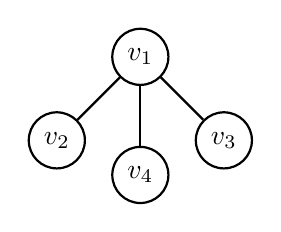
\begin{tikzpicture}[node distance={15mm}, thick, main/.style = {draw, circle}] 
\node[main] (1) {$v_1$}; 
\node[main] (2) [below left of=1] {$v_2$}; 
\node[main] (3) [below right of=1] {$v_3$}; 
\node[main] (4) [below of=1] {$v_4$}; 
\draw (1) -- (2); 
\draw (1) -- (3); 
\draw (1) -- (4); 
\end{tikzpicture}
\caption{Friends structure 1} \label{fig:Figure1}
\end{figure} 

Consider the example in Figure  \ref{fig:Figure1}.  We can calculate the AFSI of  $v_1$ as:
\begin{equation*}
    \begin{split}
     I_{v_1}^{AvgFSI}(C^{r}) &= \frac{1}{\vert F_{v_1} \vert}\cdot \sum_{v_j\in {F_{v_i}}}  \beta_{v_j}(C^{r})\\
                 &= \frac{1}{3}\cdot \big(  \beta_{v_2}(C^{r}) +  \beta_{v_3}(C^{r}) +  \beta_{v_4}(C^{r}) \big) =\frac{7}{3}
\end{split}
\end{equation*}

Similarly, we can calculate the other AFSI: $ I_{v_2}^{AvgFSI}(C^{r}) = I_{v_3}^{AvgFSI}(C^{r})=I_{v_4}^{AvgFSI}(C^{r}) = 3$.
We say, for a given committee election case, for a single voter, the higher AFSI a rule can bring, the higher the altruism level this voter give to this rule. 

\subsection{Measuring altruism of each voter with the Minimum Friends Satisfaction Index (MinFSI)}
It is also meaningful to find out the minimum satisfaction of in the voter's friends circle. For voter $v_i$ after applying a voting rule $r$ and reach the final result of $C^{r}$, we denote the Minimum Friends Satisfaction Index (Min-FSI) as $I_{v_i}^{MinFSI}(C^{r})$
\begin{equation}I_{v_i}^{MinFSI}(C^{r}) =  \min \big ( \{ \beta_{v}(C^{r}): v \in F_{v_i}\}  \big)\label{si:MinFSI}
\end{equation}
For our committee election case in Figure   \ref{fig:Figure1}, we can calculate $I_{v_1}^{MinFSI}(C^{r}) = 1$, $I_{v_2}^{MinFSI}(C^{r}) =3$, $I_{v_3}^{MinFSI}(C^{r}) = 3$ , $I_{v_4}^{MinFSI}(C^{r}) =3$.


\subsection{Measuring altruism of each voter with the Maximum Friends Satisfaction Index (MaxFSI)}

Similarly we can find out the maximum satisfaction of in the voter's friends circle. For voter
\begin{equation}I_{v_i}^{MaxFSI}(C^{r}) =  \max \big ( \{ \beta_{v}(C^{r}): v \in F_{v_i}\}  \big)\label{si:MaxFSI}
\end{equation}
For our committee election case in Figure   \ref{fig:Figure1}, we can calculate $I_{v_1}^{MaxFSI}(C^{r}) = 3$, $I_{v_2}^{MaxFSI}(C^{r}) =3$, $I_{v_3}^{MaxFSI}(C^{r}) = 3$ , $I_{v_4}^{MaxFSI}(C^{r}) =3$.



\subsection{Measuring the aggregated Satisfaction Index}
After we have considered the single voter FSI value, we now take a look at all voters aggregated and evaluate our voting rules also depending on the overall FSI scores.  For this, we will look at the different options shown in the table \ref{tab:aggregation_options}. In the chapter, we will introduce all these criterion one after another.


\begin{table}[h]
    \centering
    \begin{tabular}{{ p{4cm}p{2.7cm}p{2,7cm}p{2.7cm}  }} 
    \diagbox[dir =SE]{Single}{Aggregated}&  Average&  Minimum& Maximum\\ 
         Average&  $I^{Avg-Avg}(C^{r})$&  $I^{Min-Avg}(C^{r})$& $I^{Max-Avg}(C^{r})$\\ 
         Minimum&  $I^{Avg-Min}(C^{r})$&  $I^{Min-Min}(C^{r})$& $I^{Max-Min}(C^{r})$\\ 
         Maximum&  $I^{Avg-Max}(C^{r})$&  $I^{Min-Max}(C^{r})$& $I^{Max-Max}(C^{r})$\\ 
    \end{tabular}
    \caption{Aggregation options}
    \label{tab:aggregation_options}
\end{table}
We first consider the average, minimum and maximum of the AvgFSI of all voters for a voting rule $r$ in a committee election case $E(C,V,k)$,  where $m = \vert C \vert, n= \vert V \vert$. As we mentioned earlier, we denote $C^{r}$ as the final election result achieved by applying rule $r$:
\begin{equation}
     I^{Avg-AvgFSI}(C^{r}) = \frac{1}{n}\cdot \sum_{j=1}^{n} I_{v_j}^{AvgFSI}(C^{r})
\end{equation}\begin{equation}
     I^{Min-AvgFSI}(C^{r}) = \min \big ( \{I_{v}^{AvgFSI}(C^{r}): v \in V\}  \big) 
\end{equation}
\begin{equation}
     I^{Max-AvgFSI}(C^{r}) = \max \big ( \{I_{v}^{AvgFSI}(C^{r}): v \in V\}  \big) 
\end{equation}


For our committee election case in Figure   \ref{fig:Figure1}, we can calculate:
\begin{equation*}
 I^{Avg-AvgFSI}(C^{r}) = \frac{17}{6},  I^{Min-AvgFSI}(C^{r}) = \frac{7}{3},  I^{Max-AvgFSI}(C^{r}) = 3
 \end{equation*}
Then we will consider the average, minimum and maximum of the MinFSI among all voters:

\begin{equation}
     I^{Avg-MinFSI}(C^{r}) = \frac{1}{n}\cdot \sum_{j=1}^{n} I_{v_j}^{MinFSI}(C^{r})
\end{equation}
\begin{equation}
     I^{Min-MinFSI}(C^{r}) = \min \big ( \{I_{v}^{MinFSI}(C^{r}): v \in V\}  \big) 
\end{equation}
\begin{equation}
     I^{Max-MinFSI}(C^{r}) = \max \big ( \{I_{v}^{MinFSI}(C^{r}): v \in V\}  \big) 
\end{equation}
For our committee election case in Figure   \ref{fig:Figure1}, we can calculate:

\begin{equation*}
 I^{Avg-AvgFSI}(C^{r}) = \frac{5}{2}, I^{Min-MinFSI}(C^{r}) = 1,  I^{Max-MinFSI}(C^{r}) = 3
 \end{equation*}

Finally we will consider the average, minimum and maximum of the MaxFSI among all voters:
\begin{equation}
     I^{Avg-MaxFSI}(C^{r}) = \frac{1}{n}\cdot \sum_{j=1}^{n} I_{v_j}^{MaxFSI}(C^{r})
\end{equation}
\begin{equation}
     I^{Min-MaxFSI}(C^{r}) = \min \big ( \{I_{v}^{MaxFSI}(C^{r}): v \in V\}  \big) 
\end{equation}
\begin{equation}
     I^{Max-MaxFSI}(C^{r}) = \max \big ( \{I^{MaxFSI}(C^{r}): v \in V\}  \big) 
\end{equation}For our committee election case in Figure   \ref{fig:Figure1}, we can calculate:\begin{equation*}
    I^{Avg-MaxFSI}(C^{r}) = 3, I^{Min-MaxFSI}(C^{r}) = 3, I^{Max-MaxFSI}(C^{r}) = 3
\end{equation*}

\subsection{A concrete example to show the difference between the measurements}
The election is as follows:  $E(C,V,3)$,  where the set of candidates is $ C = \{c_a,c_b,c_c,c_d,c_e,c_f\}$, the set of voters is $V = \{v_1,v_2,v_3,v_4,v_5,v_6\}$  and $ m = 6, n = 6$ with the friend structure represented in Figure \ref{fig:Figure2}.  The preferences of the voters are respectively

\begin{align*}
\succeq_{v_1} =  \{c_a\succeq c_b \succeq c_c\succeq c_d\succeq c_e\succeq c_f\},\\  \succeq_{v_2} =  \{c_b\succeq c_d \succeq c_e\succeq c_c\succeq c_f\succeq c_a\},\\ \succeq_{v_3} =  \{c_f\succeq c_e \succeq c_b\succeq c_a\succeq c_d\succeq c_c\}, \\\succeq_{v_4} =  \{c_d\succeq c_c \succeq c_a\succeq c_f\succeq c_b\succeq c_e\},\\\succeq_{v_1} =  \{c_c\succeq c_a \succeq c_f\succeq c_e\succeq c_d\succeq c_b\},\\\succeq_{v_1} =  \{c_e\succeq c_f \succeq c_d\succeq c_b\succeq c_a\succeq c_c\}. 
\end{align*}
\theoremstyle{definition}
\newtheorem{example}{Example}[section]

\begin{example}
\begin{figure}[h]
\centering
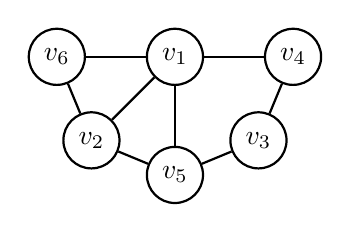
\begin{tikzpicture}[node distance={15mm}, thick, main/.style = {draw, circle}] 
\node[main] (1) {$v_1$}; 
\node[main] (2) [below left of=1] {$v_2$}; 
\node[main] (3) [below right of=1] {$v_3$}; 
\node[main] (4) [right of=1] {$v_4$}; 
\node[main] (5) [below of=1] {$v_5$}; 
\node[main] (6) [left of=1] {$v_6$}; 
\draw (1) -- (6); 
\draw (1) -- (2); 
\draw (1) -- (4); 
\draw (1) -- (5); 
\draw (2) -- (5); 
\draw (2) -- (6); 
\draw (3) -- (4); 
\draw (3) -- (5); 
\end{tikzpicture}
\caption{Friends structure with 6 voters-1} \label{fig:Figure2}
\end{figure}

\begin{figure}[h]
\centering
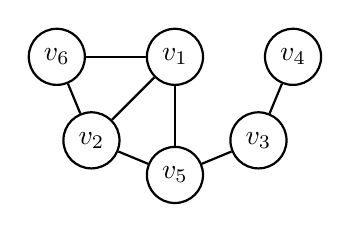
\begin{tikzpicture}[node distance={15mm}, thick, main/.style = {draw, circle}] 
\node[main] (1) {$v_1$}; 
\node[main] (2) [below left of=1] {$v_2$}; 
\node[main] (3) [below right of=1] {$v_3$}; 
\node[main] (4) [right of=1] {$v_4$}; 
\node[main] (5) [below of=1] {$v_5$}; 
\node[main] (6) [left of=1] {$v_6$}; 
\draw (1) -- (6); 
\draw (1) -- (2); 
\draw (1) -- (5); 
\draw (2) -- (5); 
\draw (2) -- (6); 
\draw (3) -- (4); 
\draw (3) -- (5); 
\end{tikzpicture}
\caption{Friends structure with 6 voters-2} \label{fig:Figure3}
\end{figure}

Concretely we take an example with friends structure of Figure \ref{fig:Figure2} and show how all these measurements are to be calculated and all of them are different. 
\end{example}

We can start with calculating the Borda Score  and the single voter FSIs of the voted committee from each voter with Equations \ref{con:bordascore}, \ref{si:AvgFSI}, \ref{si:MinFSI}, \ref{si:MaxFSI}. 
With this example, we can find out that all of the proposed measuring means are of different types and can result in different values. 

We iterate throw all the possible committee in order to find the best committee under each measuring methods. We number the possible committee as follows:
    

\begin{table}[h]
                        \caption{List of all possible committees}
    \centering
    \begin{tabular}{ccc}
         &$1. (c_a, c_b, c_c)$&$2. (c_a, c_b, c_d)$\\
         &$3.(c_a,c_b, c_e)$&$4. (c_a, c_b, c_f)$\\
         &$5. (c_a, c_c,c_d)$&$6. (c_a, c_c, c_e)$\\
         &$7. (c_a, c_c, c_f)$&$8. (c_a, c_d, c_e)$\\
         &$9. (c_a, c_d, c_f)$&$10. (c_a, c_e, c_f)$\\
         &$11. (c_b, c_c, c_d)$&$12. (c_b, c_c, c_e)$\\
         &$13.(c_b, c_c, c_f)$&$14. (c_b, c_d, c_e)$\\
         &$15.(c_b, c_d, c_f)$&$16. (c_b, c_e, c_f)$\\
         &$17. (c_c, c_d, c_e)$&$18.(c_c, c_d, c_f)$\\
         &$19. (c_c, c_e, c_f)$&$20.(c_d, c_e, c_f)$\\
    \end{tabular}
    
    \label{tab:my_label}
\end{table}
If we consider the friends structure of Figure \ref{fig:Figure2}. We can use the 9 measuring methods and come to the conclusion that for each of these methods, the following committee will be the best committee as in Table \ref{tab:res_table_1}:

\begin{table}[h] 
\caption{Ideal committee - committee number - structure 1 }
    \centering
     \centering
        \begin{tabular}{ccccc}
             $avg-avg$&  $min-avg$&  $max-avg$&  $avg-min$& $min-min$\\
             0&  11&  0&  1& 7\\
             $max-min$&  $avg-max$&  $min-max$&  $max-max$& \\
             0&  4&  1&  0& \\
    \end{tabular}
  
    \label{tab:res_table_1}
\end{table}
If we consider the friends structure of Figure \ref{fig:Figure3}. The following committee will be the best committee as in Table \ref{tab:res_table_2}:


    \begin{table}[h]
    \caption{Ideal committee - committee number - structure 2}
        \centering
        \begin{tabular}{ccccc}
             $avg-avg$&  $min-avg$&  $max-avg$&  $avg-min$& $min-min$\\
             3&  15&  15&  0& 15\\
             $max-min$&  $avg-max$&  $min-max$&  $max-max$& \\
             11&  0&  12&  7& \\
        \end{tabular}
     
        \label{tab:res_table_2}
    \end{table}    

This way, we can find out that all of these methods are optimising to different results and are not dependent of each other.


\subsection{Finding the best committee as ILP Problems}

To find the best committee for the different measuring methods can be very time consuming. Therefore we want to turn them into ILP problems and user existing solver Gurobi to accelerate the calculation. For each of the measuring methods we mentioned in the above chapter, we developed a corresponding ILP model.and explain them in this chapter.

\subsubsection*{Common Input}
Input: A committee election case $E (C,V,k)$ where $\vert C \vert =m $, $\vert V \vert =n$, A graph $G(V,E)$ to represent the relationship between the voters. The preference of each voter towards all candidates.

\paragraph*{ILP Problem 1: Maximizing  $I^{Avg-Avg}(C^{r})$}
\
\begin{itemize}
  \item \textbf{Variables}: 

\textbf{A set of binary decision variables $x_i$:} \[ \bigg\{ x_i \in \{0, 1\} \bigg\}_{i=1}^m \] The value of $x_i$ represents the status of candidate $c_i$, \(x_i = 1\) indicates choosing $c_i$ and \(x_i = 0\) indicates not choosing $c_i$.


\textbf{A continuous decision variables $s$:} 
\[ \bigg\{ s\in \mathbb{Q}_{\geq 0} \bigg\}\] 
$s$ represents the value of $I^{Avg-Avg}(C^{r})$.
    \item \textbf{Constraints}:
The constraint requires that the sum of binary decision variables \(x_1, x_2, \ldots, x_m\) equals the committee size of the election \(k\), represented as:
\begin{equation} \sum_{i=1}^m x_i = k     \label{eq:ilpavgavg1}
\end{equation}

To reformulate $s$:
\begin{equation}
\begin{split}
 s & = \sum_{i=1}^{n} I_{v_i}^{AvgFSI}(C^{r})  = I_{v_1}^{AvgFSI}(C^{r}) + I_{v_2}^{AvgFSI}(C^{r}) +\dots+I_{v_n}^{AvgFSI}(C^{r}) \\
& =  \frac{1}{\vert F_{v_1} \vert}\cdot \Big( f_{v_1}^{rel}(v_1) \cdot \beta_{v_1}(C^{r})+\dots+f_{v_1}^{rel}(v_n) \cdot \beta_{v_n}(C^{r})\Big)\\
& +\dots \\
& +\frac{1}{\vert F_{v_n} \vert}\cdot \Big(f_{v_n}^{rel}(v_1) \cdot \beta_{v_1}(C^{r})+\dots+f_{v_n}^{rel}(v_n) \cdot \beta_{v_n}(C^{r})\Big)\\
& = \frac{1}{\vert F_{v_1} \vert}\cdot \Big(f_{v_1}^{rel}(v_1)\cdot \big(x_1\cdot \beta_{v_1}(c_1)+x_2\cdot \beta_{v_1}(c_2)+\dots +x_n\cdot \beta_{v_1}(c_n)\big) \\
& +\dots \\
& +f_{v_1}^{rel}(v_n)\cdot \big(x_1\cdot \beta_{v_n}(c_1)+x_2\cdot \beta_{v_n}(c_2)+\dots +x_n\cdot \beta_{v_n}(c_n)\big)\Big) \\
& +\dots \\
& +\frac{1}{\vert F_{v_n} \vert}\cdot \Big(f_{v_n}^{rel}(v_1)\cdot \big(x_1\cdot \beta_{v_1}(c_1)+x_2\cdot \beta_{v_1}(c_2)+\dots +x_n\cdot \beta_{v_1}(c_n)\big) \\
& +\dots \\
& +f_{v_n}^{rel}(v_n)\cdot \big(x_1\cdot \beta_{v_n}(c_1)+x_2\cdot \beta_{v_n}(c_2)+\dots +x_n\cdot \beta_{v_n}(c_n)\big)\Big)
\end{split}
\end{equation}
  
  \item  \textbf{Objective function:}
  \[\text{maximize} \quad s\]

 \item  \textbf{Explanation:}
Constraint \ref{eq:ilpavgavg1} ensures that the number of selected candidates in the committee \(C^r\) is exactly \(k\). This constraint guarantees that the committee size is fixed and meets the required number of candidates. \(s\) represents the value of $I^{Avg-Avg}(C^{r})$ if a preferred committee \(C^r\) is to win the election. Maximizing \(s\) in a feasible ILP solution ensures that \(s\) provides the maximum value of \(I^{Avg-Avg}(C^{r})\). 

If there exists a feasible solution to this ILP where all constraints are satisfied and \(s\) is maximized, then \(s\) will indeed give us the maximum value of \(I^{Avg-Avg}(C^{r})\). This means that the selected committee \(C^r\) optimally meets the requirements set by the ILP formulation, ensuring both the fixed committee size \(k\) and the maximum of the average FSI. 
\end{itemize}

\paragraph*{ILP Problem 2: Maximizing $I^{Min-Avg}(C^{r})$}\mbox{} \\

\begin{itemize}
  \item \textbf{Variables}: 

\textbf{A set of binary decision variables $x_i$:} \[ \bigg\{ x_i \in \{0, 1\} \bigg\}_{i=1}^m \] The value of $x_i$ represents the status of candidate $c_i$, \(x_i = 1\) indicates choosing $c_i$ and \(x_i = 0\) indicates not choosing $c_i$.


\textbf{A continuous decision variables $s$:} 
\[ \bigg\{ s\in \mathbb{Q}_{\geq 0} \bigg\}\] 
$s_i$ represents the value of $I_{v_i}^{Avg}(C^{r})$.
    \item \textbf{Constraints}:
The constraint requires that the sum of binary decision variables \(x_1, x_2, \ldots, x_m\) equals the committee size of the election \(k\), represented as:
\begin{equation} \sum_{i=1}^m x_i = k     \label{eq:ilpminavg1}
\end{equation}

To further constraint $s$, for all $v_i$ the following constraint inequality holds:
\begin{equation}\forall v_i \in V, \quad
 s \leq \frac{1}{\vert F_{v_i} \vert}\cdot \Big(f_{v_i}^{rel}(v_1) \cdot \beta_{v_1}(C^{r})+\dots+f_{v_i}^{rel}(v_n) \cdot \beta_{v_i}(C^{r})\Big)    \label{eq:ilpminavg2}
\end{equation}
  
  \item  \textbf{Objective function:}
  \[\text{maximize} \quad s\]





 \item  \textbf{Explanation:}
Constraint \ref{eq:ilpminavg1} ensures that the number of selected candidates in the committee \(C^r\) is exactly \(k\). This constraint guarantees that the committee size is fixed and meets the required number of candidates. 

\(s\) serves as the lower bound of $I^{Min-Avg}(C^{r})$ if a preferred committee \(C^r\) is to win the election. Constraint \ref{eq:ilpminavg2} ensures that $s$ is the lower bound of all \(I_{v_i}^{Avg}(C^{r})\). Maximizing \(s\) in a feasible ILP solution ensures that \(s\) provides the maximum value of \(I^{Min-Avg}(C^{r})\). 

If there exists a feasible solution to this ILP where all constraints are satisfied and \(s\) is maximized, then \(s\) will indeed give us the maximum value of \(I^{Min-Avg}(C^{r})\). This means that the selected committee \(C^r\) optimally meets the requirements set by the ILP formulation, ensuring both the fixed committee size \(k\) and the minimum of the average FSI. 






\end{itemize}
















\paragraph*{ILP Problem 3: Maximizing  $I^{Avg-Max}(C^{r})$}

\begin{itemize}

  \item \textbf{Variables}: 

\textbf{A set of binary decision variables $x_i$:} \[ \bigg\{ x_i \in \{0, 1\} \bigg\}_{i=1}^m \] The value of $x_i$ represents the status of candidate $c_i$, \(x_i = 1\) indicates choosing $c_i$ and \(x_i = 0\) indicates not choosing $c_i$.


\textbf{A set of two-dimensional binary decision variables \( a_{ij} \):}
\[
\{ a_{ij} \mid 1 \leq i \leq |V|, \quad 1 \leq j \leq |F_{vi}| \},  (i, j \in \mathbb{N})
\]

\textbf{A set of continuous decision variables $s_i$:} 
\[ \bigg\{ s_i \in \mathbb{Q}_{\geq 0} \bigg\}_{i=1}^n \] 
$s_i$ represents the value of $I_{v_i}^{MaxFSI}$ of \(v_i\).
    \item \textbf{Constraints}:
The constraint requires that the sum of binary decision variables \(x_1, x_2, \ldots, x_m\) equals the committee size of the election \(k\), represented as:
\begin{equation} \sum_{i=1}^m x_i = k \label{eq:ilpavgmax1}
\end{equation}

For each \(i\) with \(1 \leq i \leq |V|\), the constraint is that the sum of \( a_{ij} \) for all \( j \in F_{vi} \) (where \( i \) belongs to the set \( V \)) equals 1.:
\begin{equation} \forall i \in \{1, 2, \ldots, |V|\}, \quad \sum_{j=1}^{|F_{vi}|} a_{ij} = 1 \label{eq:ilpavgmax2}
\end{equation}

To further constraint $s_i$ as the $I_{v_i}^{MaxFSI}$, we introduce a very big value $M$, in our case $M \geq  2m$. For all \( i \in \{1, 2, \ldots, |V|\} \) and for each  \( j \in \{1, 2, \ldots, |\text{F}_{v_i}|\} \), the following constraint inequality holds:
\begin{equation} \beta_{F_{v_i}(j)}(C^{r}) + (1 - a_{ij})\cdot M \geq s_i \label{eq:ilpavgmax3}
\end{equation}
  
  \item  \textbf{Objective function:}
  \begin{equation}\text{maximize} \quad \frac{\sum_{i=1}^{n} s_i}{n}    \label{eq:ilpavgmax4}
\end{equation}


\item  \textbf{Explanation:}
Constraint \ref{eq:ilpavgmax1} ensures that the number of selected candidates in the committee \(C^r\) is exactly \(k\). This constraint guarantees that the committee size is fixed and meets the required number of candidates.
Constraint \ref{eq:ilpavgmax2} guarantees that only one friend of each voter is selected for getting the maximized FSI.
Constraint \ref{eq:ilpavgmax3} indicates that \(s\) serves as a upper bound of the highest FSI given by a voter's friend if a preferred committee \(C^r\) win the election.
The objective function \ref{eq:ilpavgmax4} represents the $I^{Avg-Max}(C^{r})$ over all voters. Maximizing  the objective function in a feasible ILP solution ensures that the ILP provides the maximum value of \(I^{Avg-Max}(C^{r})\), representing the average FSI among the most satisfied friends of each voter given by a winning committee \(C^r\)in the election. 

If there exists a feasible solution to this ILP where all constraints are satisfied and the objective function is maximized, then the ILP will indeed give us the maximum value of \(I^{Avg-Max}(C^{r})\). This means that the selected committee \(C^r\) optimally meets the requirements set by the ILP formulation, ensuring both the fixed committee size \(k\) and is the upper bound of the average FSI value of the most satisfied friends. 

\end{itemize}


\paragraph*{ILP Problem 4: Maximizing  $I^{Max-Max}(C^{r})$}\mbox{} \\

For this we will do the optimization of the $I_{v_i}^{Max}(C^{r})$ for each voter $v_i$. Afterwards, we will iterate through all the $I_{v_i}^{Max}(C^{r})$ and find the maximum value:
  \[I^{Max-Max}(C^{r}) = \max\{ I_{v_1}^{Max}(C^{r}), I_{v_2}^{Max}(C^{r}), \ldots, I_{v_n}^{Max}(C^{r}) \}\]
\begin{itemize}

  \item \textbf{Variables}: 

\textbf{A set of binary decision variables $x_i$:} \[ \bigg\{ x_i \in \{0, 1\} \bigg\}_{i=1}^m \] The value of $x_i$ represents the status of candidate $c_i$, \(x_i = 1\) indicates choosing $c_i$ and \(x_i = 0\) indicates not choosing $c_i$.


\textbf{A set of two-dimensional binary decision variables \( a_{ij} \):}
\[
\{ a_{ij} \mid 1 \leq i \leq |V|, \quad 1 \leq j \leq |F_{vi}| \},  (i, j \in \mathbb{N})
\]

\textbf{A set of continuous decision variables $s$:} 
\[ \bigg\{ s \in \mathbb{Q}_{\geq 0} \bigg\} \] 
$s$ represents the value of $I^{Max-Max}$ .
    \item \textbf{Constraints}:
The constraint requires that the sum of binary decision variables \(x_1, x_2, \ldots, x_m\) equals the committee size of the election \(k\), represented as:
\begin{equation} \sum_{i=1}^m x_i = k     \label{eq:ilpmaxmax1}
\end{equation}

For each \(i\) with \(1 \leq i \leq |V|\), the constraint is that the sum of \( a_{ij} \) for all \( j \in F_{vi} \) (where \( i \) belongs to the set \( V \)) equals 1.:
\begin{equation} \forall i \in \{1, 2, \ldots, |V|\}, \quad \sum_{j=1}^{|F_{vi}|} a_{ij} = 1  \label{eq:ilpmaxmax2}
\end{equation}

To further constraint $s$ as the $I^{Max-Max}$, we introduce a very big value $M$, in our case $M \geq  2m$. For all \( i \in \{1, 2, \ldots, |V|\} \) and for each  \( j \in \{1, 2, \ldots, |\text{F}_{v_i}|\} \), the following constraint inequality holds:
\begin{equation} \beta_{F_{v_i}(j)}(C^{r}) + (1 - a_{ij})\cdot M \geq s \label{eq:ilpmaxmax3}
\end{equation}
  
  \item  \textbf{Objective function:}
  \[\text{maximize} \quad s \]

\item  \textbf{Explanation:}
Constraint \ref{eq:ilpmaxmax1} ensures that the number of selected candidates in the committee \(C^r\) is exactly \(k\). This constraint guarantees that the committee size is fixed and meets the required number of candidates.
Constraint \ref{eq:ilpmaxmax2} guarantees that only one friend of each voter is selected for getting the maximized FSI.
Constraint \ref{eq:ilpmaxmax3} indicates that \(s\) represents the upper bounded FSI given by a voter's friend if a preferred committee \(C^r\) win the election. Maximizing \(s\) in a feasible ILP solution ensures that \(s\) provides the maximum value of \(I_{v_i}^{Max}(C^{r})\), representing the maximun FSI a voter can reach given by a winning committee \(C^r\)in the election. 

If there exists a feasible solution to this ILP where all constraints are satisfied and \(s\) is maximized, then \(s\) will indeed give us the maximum value of \(I_{v_i}^{Max}(C^{r})\). This means that the selected committee \(C^r\) optimally meets the requirements set by the ILP formulation, ensuring both the fixed committee size \(k\) and the maximum of the most satisfied friends. Afterwards, we gether the result for each voter $v_i$ and retrieve the highest score among all voters. This will give the $I^{Max-Max}(C^{r})$ over all voters.

\end{itemize}


\paragraph*{ILP Problem 5: Maximizing  $I^{Avg-Min}(C^{r})$}

\begin{itemize}

  \item \textbf{Variables}: 

\textbf{A set of binary decision variables $x_i$:} \[ \bigg\{ x_i \in \{0, 1\} \bigg\}_{i=1}^m \] The value of $x_i$ represents the status of candidate $c_i$, \(x_i = 1\) indicates choosing $c_i$ and \(x_i = 0\) indicates not choosing $c_i$.

\textbf{A set of continuous decision variables $s_i$:} 
\[ \bigg\{ s_i \in \mathbb{Q}_{\geq 0} \bigg\}_{i=1}^n \] 
$s_i$ represents the value of $I_{v_i}^{MinFSI}$ of \(v_i\).
    \item \textbf{Constraints}:
The constraint requires that the sum of binary decision variables \(x_1, x_2, \ldots, x_m\) equals the committee size of the election \(k\), represented as:
\begin{equation} \sum_{i=1}^m x_i = k \label{eq:ilpavgmin1}
\end{equation}

To further constraint $s_i$, the following constraint inequality holds:
\begin{equation} \beta_{F_{v_i}(j)}(C^{r}) \geq s_i  \label{eq:ilpavgmin2}
\end{equation}
  
  \item  \textbf{Objective function:}
  \begin{equation}\text{maximize} \quad \frac{\sum_{i=1}^{n} s_i}{n} \label{eq:ilpavgmin3}
\end{equation}
\item  \textbf{Explanation:}
Constraint \ref{eq:ilpavgmin1} ensures that the number of selected candidates in the committee \(C^r\) is exactly \(k\). This constraint guarantees that the committee size is fixed and meets the required number of candidates.
Constraint \ref{eq:ilpavgmin2} indicates that \(s\) serves as a lower bound of each voter's FSI given by all his friends if a preferred committee \(C^r\) win the election.
The objective function \ref{eq:ilpavgmin3} represents the average of the $I^{Min}(C^{r})$ over all voters. Maximizing  the objective function in a feasible ILP solution ensures that the ILP provides the maximum value of \(I^{Avg-Min}(C^{r})\), representing the average FSI among the least satisfied friends of each voter given by the chosen committee \(C^r\)in the election. 

If there exists a feasible solution to this ILP where all constraints are satisfied and the objective function is maximized, then the ILP will indeed give us the maximum value of \(I^{Avg-Min}(C^{r})\). This means that the selected committee \(C^r\) optimally meets the requirements set by the ILP formulation, ensuring both the fixed committee size \(k\) and is the average of the least satisfied friends. 
\end{itemize}


\paragraph*{ILP Problem 6: Maximizing  $I^{Min-Max}(C^{r})$}

\begin{itemize}

  \item \textbf{Variables}: 

\textbf{A set of binary decision variables $x_i$:} \[ \bigg\{ x_i \in \{0, 1\} \bigg\}_{i=1}^m \] The value of $x_i$ represents the status of candidate $c_i$, \(x_i = 1\) indicates choosing $c_i$ and \(x_i = 0\) indicates not choosing $c_i$.


\textbf{A set of two-dimensional binary decision variables \( a_{ij} \):}
\[
\{ a_{ij} \mid 1 \leq i \leq |V|, \quad 1 \leq j \leq |F_{vi}| \},\quad where  (i, j \in \mathbb{N})
\]

\textbf{A set of continuous decision variables $s$:} 
\[ \bigg\{ s \in \mathbb{Q}_{\geq 0} \bigg\} \] 
$s$ represents the value of $I^{Min-Max}$ .
    \item \textbf{Constraints}:
The constraint requires that the sum of binary decision variables \(x_1, x_2, \ldots, x_m\) equals the committee size of the election \(k\), represented as:
\begin{equation} \sum_{i=1}^m x_i = k  \label{eq:ilpminmax1}
\end{equation}

For each \(i\) with \(1 \leq i \leq |V|\), the constraint is that the sum of \( a_{ij} \) for all \( j \in F_{vi} \) (where \( i \) belongs to the set \( V \)) equals 1.:
\begin{equation} \forall i \in \{1, 2, \ldots, |V|\}, \quad \sum_{j=1}^{|F_{vi}|} a_{ij} = 1  \label{eq:ilpminmax2}
\end{equation}

To further constraint $s$ as the $I^{Min-Max}$, we introduce a very big value $M$, in our case $M \geq  2m$. For all \( i \in \{1, 2, \ldots, |V|\} \) and for each  \( j \in \{1, 2, \ldots, |\text{F}_{v_i}|\} \), the following constraint inequality holds:
\begin{equation} \beta_{F_{v_i}(j)}(C^{r}) + (1 - a_{ij})\cdot M \geq s     \label{eq:ilpminmax3}
\end{equation}
  
  \item  \textbf{Objective function:}
  \[\text{maximize} \quad s \]

\item  \textbf{Explanation:}
Constraint \ref{eq:ilpminmax1} ensures that the number of selected candidates in the committee \(C^r\) is exactly \(k\). This constraint guarantees that the committee size is fixed and meets the required number of candidates.
Constraint \ref{eq:ilpminmax2} guarantees that only one friend of each voter is selected for getting the maximized FSI.
Constraint \ref{eq:ilpminmax3} indicates that \(s\) serves as a lower bound on the highest FSI given by any voter's friend if a preferred committee \(C^r\) win the election. Maximizing \(s\) in a feasible ILP solution ensures that \(s\) provides the maximum value of \(I^{Min-Max}(C^{r})\), representing the minimum FSI among the most satisfied friends of each voter given by a winning committee \(C^r\)in the election. 

If there exists a feasible solution to this ILP where all constraints are satisfied and \(s\) is maximized, then \(s\) will indeed give us the maximum value of \(I^{Min-Max}(C^{r})\). This means that the selected committee \(C^r\) optimally meets the requirements set by the ILP formulation, ensuring both the fixed committee size \(k\) and the minimum of the most satisfied friends. In this case, we make the FSI score among the most satisfied friends retain a highest possible FSI score.
\end{itemize}

\paragraph*{ILP Problem 7: Maximizing  $I^{Min-Min}(C^{r})$}

\begin{itemize}

  \item \textbf{Variables}: 

\textbf{A set of binary decision variables $x_i$:} \[ \bigg\{ x_i \in \{0, 1\} \bigg\}_{i=1}^m \] The value of $x_i$ represents the status of candidate $c_i$, \(x_i = 1\) indicates choosing $c_i$ and \(x_i = 0\) indicates not choosing $c_i$.

\textbf{A continuous decision variables $s$:} 
\[ \bigg\{ s \in \mathbb{Q}_{\geq 0} \bigg\} \] 
$s$ represents the value of $I^{Min-Min}$ .
    \item \textbf{Constraints}:
The constraint requires that the sum of binary decision variables \(x_1, x_2, \ldots, x_m\) equals the committee size of the election \(k\), represented as:

\begin{equation} \sum_{i=1}^m x_i = k     \label{eq:ilpminmin1}
\end{equation}


To further constraint $s$, assuming $C^r$ is every possible committee in the size of $k$, the following constraint inequality holds:
\begin{equation}  \beta_{F_{v_i}(j)}(C^{r}) \geq s     \label{eq:ilpminmin2}
\end{equation}

  
  \item  \textbf{Objective function:}
  \[\text{maximize} \quad s \]

 \item  \textbf{Explanation:}
Constraint \ref{eq:ilpminmin1} ensures that the number of selected candidates in the committee \(C^r\) is exactly \(k\). This constraint guarantees that the committee size is fixed and meets the required number of candidates.

Constraint \ref{eq:ilpminmin2} indicates that \(s\) serves as a lower bound on the lowest FSI required by any voter's friend preferred committee \(C^r\) to win the election, based on voter preferences. Maximizing \(s\) in a feasible ILP solution ensures that \(s\) provides the maximum value of \(I^{Min-Min}(C^{r})\), representing the minimum FSI of the least satisfied friend among all voters of a winning committee \(C^r\)in the election. 

If there exists a feasible solution to this ILP where all constraints are satisfied and \(s\) is maximized, then \(s\) will indeed give us the maximum value of \(I^{Min-Min}(C^{r})\). This means that the selected committee \(C^r\) optimally meets the requirements set by the ILP formulation, ensuring both the fixed committee size \(k\) and the minimum of the least satisfied friends. In this case, we make the least satisfied friend, as happy as possible.
\end{itemize}
\paragraph*{ILP Problem 8: Maximizing  $I^{Max-Min}(C^{r})$}\mbox{} \\
For this we will do the optimization of the $I_{v_i}^{Min}(C^{r})$ for each voter $v_i$. Afterwards, we will iterate through all the $I_{v_i}^{Min}(C^{r})$ and find the maximum value:
  \[I^{Max-Min}(C^{r}) = \max\{ I_{v_1}^{Min}(C^{r}), I_{v_2}^{Min}(C^{r}), \ldots, I_{v_n}^{Min}(C^{r}) \}\]
\begin{itemize}
  \item \textbf{Variables}: 

\textbf{A set of binary decision variables $x_i$:} \[ \bigg\{ x_i \in \{0, 1\} \bigg\}_{i=1}^m \] The value of $x_i$ represents the status of candidate $c_i$, \(x_i = 1\) indicates choosing $c_i$ and \(x_i = 0\) indicates not choosing $c_i$.


\textbf{A continuous decision variables $s$:} 
\[ \bigg\{ s\in \mathbb{Q}_{\geq 0} \bigg\}\] 
$s$ represents the value of $I_{v_i}^{MinFSI}$.
    \item \textbf{Constraints}:
The constraint requires that the sum of binary decision variables \(x_1, x_2, \ldots, x_m\) equals the committee size of the election \(k\), represented as:
\begin{equation} \sum_{i=1}^m x_i = k     \label{eq:ilpmaxmin1}
\end{equation}

To further constraint $s$, for all \( j \in F_{vi} \) the following constraint inequality holds:
\begin{equation} \beta_{F_{v_i}(j)}(C^{r}) \geq s  \label{eq:ilpmaxmin2}
\end{equation}
  
  \item  \textbf{Objective function:}
  \[\text{maximize} \quad s\]

  \item  \textbf{Explanation:}
Constraint \ref{eq:ilpmaxmin1} ensures that the number of selected candidates in the committee \(C^r\) is exactly \(k\). This constraint guarantees that the committee size is fixed and meets the required number of candidates.

Constraint \ref{eq:ilpmaxmin2} indicates that \(s\) serves as a lower bound of the smallest FSI given by each friend of the voter if a preferred committee \(C^r\) to win the election. Maximizing \(s\) in a feasible ILP solution ensures that \(s\) provides the maximum value of \(I_{v_i}^{Min}(C^{r})\), representing the minimum FSI of the least satisfied friend of $v_i$. 

If there exists a feasible solution to this ILP where all constraints are satisfied and \(s\) is maximized, then \(s\) will indeed give us the maximum value of  \(I_{v_i}^{Min}(C^{r})\). This means that the selected committee \(C^r\) optimally meets the requirements set by the ILP formulation, ensuring both the fixed committee size \(k\) and the minimum of the FSI. Afterwards, we gether the result for each voter $v_i$ and retrieve the highest score among all voters. This will give the $I^{Max-Min}(C^{r})$ over all voters.
\end{itemize}

\paragraph*{ILP Problem 9: Maximizing  $I^{Max-Avg}(C^{r})$}\mbox{} \\
For this we will do the optimization of the $I_{v_i}^{Avg}(C^{r})$ for each voter $v_i$. Afterwards, we will iterate through all the $I_{v_i}^{Avg}(C^{r})$ and find the maximum value:
  \[I^{Max-Avg}(C^{r}) = \max\{ I_{v_1}^{Avg}(C^{r}), I_{v_2}^{Avg}(C^{r}), \ldots, I_{v_n}^{Avg}(C^{r}) \}\]
\begin{itemize}
  \item \textbf{Variables}: 

\textbf{A set of binary decision variables $x_i$:} \[ \bigg\{ x_i \in \{0, 1\} \bigg\}_{i=1}^m \] The value of $x_i$ represents the status of candidate $c_i$, \(x_i = 1\) indicates choosing $c_i$ and \(x_i = 0\) indicates not choosing $c_i$.


\textbf{A continuous decision variables $s$:} 
\[ \bigg\{ s\in \mathbb{Q}_{\geq 0} \bigg\}\] 
$s$ represents the value of $I_{v_i}^{Avg}(C^{r})$ and can therefore be reformulated as follows:
\[ \forall v_i \in V, \quad
 s = \frac{1}{\vert F_{v_i} \vert}\cdot \Big(f_{v_i}^{rel}(v_1) \cdot \beta_{v_1}(C^{r})+\dots+f_{v_i}^{rel}(v_n) \cdot \beta_{v_i}(C^{r})\Big)\]
    \item \textbf{Constraints}:
The constraint requires that the sum of binary decision variables \(x_1, x_2, \ldots, x_m\) equals the committee size of the election \(k\), represented as:
\begin{equation} \sum_{i=1}^m x_i = k     \label{eq:ilpmaxavg1}
\end{equation}
  
  \item  \textbf{Objective function:}
  \[\text{maximize} \quad s\]

  \item  \textbf{Explanation:}
Constraint \ref{eq:ilpmaxavg1} ensures that the number of selected candidates in the committee \(C^r\) is exactly \(k\). This constraint guarantees that the committee size is fixed and meets the required number of candidates.

For each $v_i$, \(s\) serves as $I_{v_i}^{Avg}(C^{r})$ given by all friends of the $v_i$ if a preferred committee \(C^r\) is to win the election. Maximizing \(s\) in a feasible ILP solution ensures that \(s\) provides the maximum value of \(I_{v_i}^{Avg}(C^{r})\), representing the maximum of the average FSI if all friends of $v_i$. 

If there exists a feasible solution to this ILP where all constraints are satisfied and \(s\) is maximized, then \(s\) will indeed give us the maximum value of  \(I_{v_i}^{Avg}(C^{r})\). This means that the selected committee \(C^r\) optimally meets the requirements set by the ILP formulation, ensuring both the fixed committee size \(k\) and the maximum of the average FSI. Afterwards, we gether the result for each voter $v_i$ and retrieve the highest score among all voters. This will give the $I^{Max-Avg}(C^{r})$ over all voters.

\end{itemize}




\section{The different friend structures represented by graph models}
In this section, we will use different graph models to represent the friend structure between the voters within an election case. The nodes in the graph will represent the voters and the edges represent the friend relationship.  As the first step, we will generate the relationship randomly using different graph models.

\subsection{Friend structures generated according to graph models}

With the voter data from \href{https://www.preflib.org}{PrefLib} we can extract an election $E (C,V,k)$ and the preference of each voter over all the candidate We use the Erdős–Rényi (ER) model to generate a friend structure randomly. For a graph $G(p,n)$, the nodes correspond each of the voters and the friendship between voters is represented by edges,if two voters are friends, there will be an edge between them. For example in the \href{https://www.preflib.org/static/data/agh/00009-00000001.soc}{AGH Course Selection 2003}, 146 students showed Complete List of Strict Orders from 9 candidate courses. For this we can generate a graph model $G(p,146)$ with $p \in [0,1]$. We can define the $p$ value depending on the different settings of our experiment in the coming sections.

A small world graph is another graph model we use to generate our friend structure. Characterized by short average path lengths and high clustering, voters in this graph model are highly interconnected. 

We also use caveman graph model to represent another kind of social relationship between the voters. Here nodes are organized into cliques with sparse connections between the cliques. This represent a kind of social network that there are highly interconnecter communities in a society where the connection between the communities are relatively rare. 

Finally, we use scale-free graph to model the social networks between the voters. In a scale-free graph,some node with have have a significantly higher degrees then the majority of the nodes. This is similar to the real world situation with a few of the voters having a lot of friends and connections whereas others are having only simple social relationships.

\section{The research experiment}

\subsection{Research Questions}
With the measuring methods designed and the ILP models ready. We do a data analysis experiment with data instances from \href{https://www.preflib.org/}{PrefLib} in our next step. Our measuring methods are designed for instances of type SOC (Strict Orders - Complete List). We will consider the FIS for the 9 different measuring methods separately and do not mix their results. Our research questions are listed as follows:
\begin{enumerate}
    \item \textbf{Research Question 1}: How likely are the 9 methods to be different from each other?
        \newline
    For this, we will fix the PrefLib instance and the committee size and the graph type. With growing $p$ in the range $[0.1,1]$, we will compare each pair of the measuring methods and observe whether the result committee is identical or not.
    \item \textbf{Research Question 2}: Given a graph type representing the relationship between all the voters, how will the density of the graph influence the FSI values. 
    \newline
    For this we will fix the graph type, the committee size for the election and the PrefLib instance. Assuming $G(p,N)$ is a graph where $N$ is the set of all nodes and  $p$ is the likelihood how are each pair of node to be connected with an edge, represents the voters and relationship between them. If the voters are friends, there will be an edge between the corresponding nodes. We will observe the development of the FSI value under the different measuring methods respectively with growing $p$ in the range $[0.1,1]$
    
    \item \textbf{Research Question 3}: How can the different relationships between voters represented by graph types influence the committee election result and the corresponding FSI values?
    \newline
    To answer this question, we will fix the PrefLib instance and the committee size, then we will run the experiment on the different graph types. We will observe the development of the FSI value under the different measuring methods respectively with different graph types like scale-free graph, small-world network, Erdős–Rényi (ER) random graph, caveman graph model. For graph models that need to define the probability of the edge existence $p$, we will unify the $p$ for all relevant graph types, to compare with the graph type without the $p$- value predefined, we will make and explain our assumption in the experiment in detail in the section where we show the result of our experiments.
    

\end{enumerate}

\end{document}
